\section{Zielsetzung}
\label{sec:Ziel}
In diesem Versuch wird die Funktionsweise und charakteristische Eigenschaften eines \textit{Geiger-Müller-Zählrohrs} untersucht. Dabei wird die Länge des Plateubereiches
und die Totzeit des Zählrohres ermittelt.

\section{Theorie}
\label{sec:Theorie}
Das Geiger-Müller-Zählrohr wird verwendet um Strahlungsintensitäten ionisierender Strahlung zu messen. Prinzipiell ionisieren die einfallenden Teilchen (oder Lichtquanten) der 
$\alpha$-, $\beta$- oder $\gamma$-Strahlung Atome im Inneren des Zählrohres, was zu einem elektrischen Signal führt. Die genaue Funktionsweise des Geiger-Müller-Zählrohres
--auch \textit{GMZ} genannt-- wird im Folgenden beschrieben.

\subsection{Funktionsweise eines Geiger-Müller-Zählrohres}
\label{subsec:Funktion_GMZ}
Das \textit{GMZ} besteht im Wesentlichen aus einer zylinderförmigen Kathode, in dessen Zentrum ein Anodendraht verläuft. Wie die Benennung bereits suggeriert, wird eine Spannung 
an die beiden Bauteile angelegt. An der Vorderseite der Apparatur befindetr sich ein Eintrittsfenster aus Mylar, welches auch das Eindringen von leicht zu absorbierender
Strahlung (wie $\alpha$-Strahlung) ermöglicht. Der Innenraum des Zählrohres ist mit einem Gas (\textit{Zählgas}) gefüllt, welches mit Alkoholdämpfen versetzt ist. Auf die Funktion
letzterer wird später eingegangen.
Der beschriebene Aufbau des \textit{GMZ} ist in \autoref{fig:GMZ_Aufbau} dargestellt. Die Polung der anliegenden Spannung ist ebenfalls der Abbildung zu entnehmen.

\begin{figure}
    \centering
    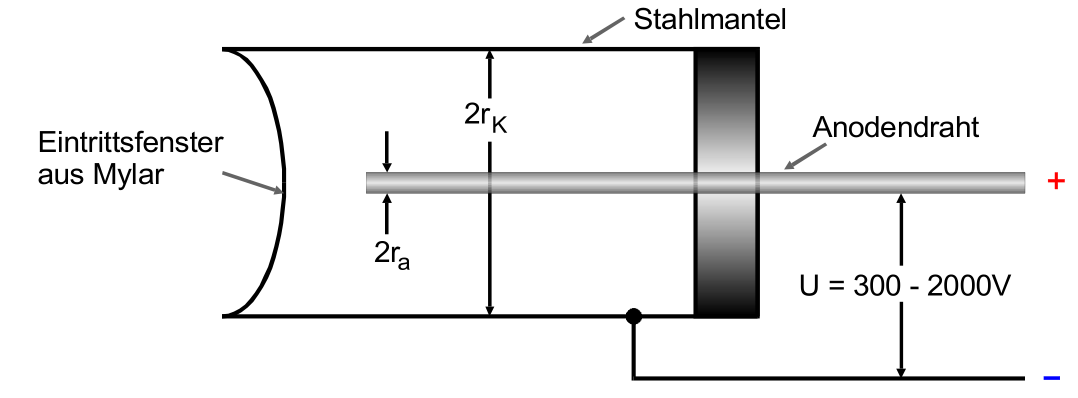
\includegraphics[width = .8\textwidth]{content/GMZ_Aufbau.png}
    \caption{Aufbau eines Geiger-Müller-Zählrohres \cite{v703}.}
    \label{fig:plot}
  \end{figure}

Wie oben bereits erwähnt, kommt es durch einfallende Strahlung zu Ionisation von Gasmolekülen. Da es vor der Absorption des Teilchens zu einer Vielzahl von Ionisationsakten
kommt, bei welchen im Mittel eine Energie von nur $\qty{26}{\electronvolt}$ abgegeben wird, ist die Anzahl der ionisierten Teilchen proportional zur Energie der Strahlung.

Die nun separierten Elektronen-Ionen Paare bewegen sich anschließend auf Grund der anliegenden Spannung in Richtung der Anode bzw. Kathode. Dabei treten abhängig von der 
Spannung verschiedene Prozesse auf.
